\let\negmedspace\undefined
\let\negthickspace\undefined
\documentclass[journal]{IEEEtran}
\usepackage[a5paper, margin=10mm, onecolumn]{geometry}
%\usepackage{lmodern} % Ensure lmodern is loaded for pdflatex
\usepackage{tfrupee} % Include tfrupee package

\setlength{\headheight}{1cm} % Set the height of the header box
\setlength{\headsep}{0mm}     % Set the distance between the header box and the top of the text

\usepackage{gvv-book}
\usepackage{gvv}
\usepackage{cite}
\usepackage{amsmath,amssymb,amsfonts,amsthm}
\usepackage{algorithmic}
\usepackage{graphicx}
\usepackage{textcomp}
\usepackage{xcolor}
\usepackage{txfonts}
\usepackage{listings}
\usepackage{enumitem}
\usepackage{mathtools}
\usepackage{gensymb}
\usepackage{comment}
\usepackage[breaklinks=true]{hyperref}
\usepackage{tkz-euclide} 
\usepackage{listings}
\def\inputGnumericTable{}                                 
\usepackage[latin1]{inputenc}                                
\usepackage{color}                                            
\usepackage{array}                                            
\usepackage{longtable}                                       
\usepackage{calc}                                             
\usepackage{multirow}                                         
\usepackage{hhline}                                           
\usepackage{ifthen}                                           
\usepackage{lscape}
\begin{document}

\bibliographystyle{IEEEtran}


\title{4.4.8}
\author{AI25BTECH11012 - GARIGE UNNATHI}
% \maketitle
% \newpage
% \bigskip
{\let\newpage\relax\maketitle}


\renewcommand{\thefigure}{\theenumi}
\renewcommand{\thetable}{\theenumi}
\setlength{\intextsep}{10pt} % Space between text and floats


\numberwithin{equation}{enumi}
\numberwithin{figure}{enumi}

\vspace{-1cm}

\textbf{Question}:\\
Find the value of x such that the four points A(x,5,-1), B(3,2,1), C(4,5,5), and
D(4,2,-2) are coplanar.


\textbf{Solution: }

 \begin{table}[h!]    
      \centering
      \begin{tabular}{|c|c|}
\hline
\textbf{Name} & \textbf{Value} \\ \hline
$\vec{A}$ & $\myvec{2 & 1 \\0 & 3}$ \\ \hline
\end{tabular}

      \caption{Variables Used}
      \label{}
    \end{table}

The equation of a plane can be given by the formula :
         
\begin{align}
    n^{T}\vec{x} = 1\\
    or\\
    x^{T}n =1 
\end{align}

Since all the points A,B,C,D are on the plane :
\begin{align}
   A^{T}n =1 \quad  B^{T}n =1 \quad  C^{T}n =1 \quad  D^{T}n =1 
\end{align}

To find $\vec{D}$ we find $\vec{n}$ :\\
Combining the above equation we get :


\begin{align}
  \myvec{B \\ C \\ D}^{T}n  = \myvec{3 & 2 & 1\\
                                     4 & 5  &  5 \\
                                     4 & 2 &-2}n  = \myvec{1\\1\\1}
\end{align}


solving the equation by row reduction we get 
\begin{align}
	\vec{n} = \myvec{\frac{9}{16} \\ -\frac{7}{16} \\ \frac{3}{16}} = \frac{1}{16}\myvec{9 \\ -7 \\ 3}
\end{align}

substituting in the equation $A^{T}n =1 $ we get:

\begin{align}
    \myvec{x & 5 &-1}\myvec{9\\-7\\3} = 16\\
    9x - 35 - 3 = 16 \\
    9x = 54
\end{align}
\begin{align}
    x = 6
\end{align}


\begin{figure}[h!]
   \centering
   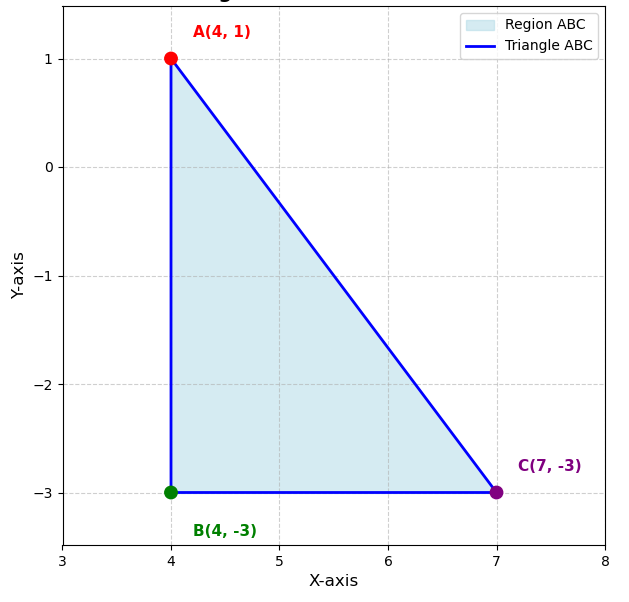
\includegraphics[width=0.7\linewidth]{/Users/unnathi/Documents/ee1030-2025/ai25btech11012/matgeo/4.4.8/figs/fig.png}
   \caption{}
   \label{stemplot}
\end{figure}


\end{document}


